% Template for CAD in medical imaging - Project Report
%          spconf.sty  - ICASSP/ICIP LaTeX style file, and
%          IEEEbib.bst - IEEE bibliography style file.
% --------------------------------------------------------------------------
\documentclass{article}
\usepackage{spconf,amsmath,graphicx}
\usepackage{subfigure}

% Title
\title{Computer Aided Diagnosis\\LUNA16: Candidate detection}
%
\makeatletter
\def\@name{ \emph{Luc Nies (s4136748)}, \emph{Tom van de Poll (s4106512)}, \emph{Harmen Prins (s4132297)}, \\ \emph{Steven Reitsma (s4132343)} \& \emph{Inez Wijnands (s4149696)}}
\makeatother

\address{Radboud University Nijmegen}
%
% For example:
% ------------
%\address{School\\
%	Department\\
%	Address}
%
% Two addresses (uncomment and modify for two-address case).
% ----------------------------------------------------------
%\twoauthors
%  {A. Author-one, B. Author-two\sthanks{Thanks to XYZ agency for funding.}}
%	{School A-B\\
%	Department A-B\\
%	Address A-B}
%  {C. Author-three, D. Author-four\sthanks{The fourth author performed the work
%	while at ...}}
%	{School C-D\\
%	Department C-D\\
%	Address C-D}
%
% More than two addresses
% -----------------------
% \name{Author Name$^{\star \dagger}$ \qquad Author Name$^{\star}$ \qquad Author Name$^{\dagger}$}
%
% \address{$^{\star}$ Affiliation Number One \\
%     $^{\dagger}$}Affiliation Number Two
%
\begin{document}
%\ninept
%
\maketitle
%
\begin{abstract}
Write your abstract here.
\end{abstract}


% Introduction
\section{Introduction}
\label{sec:intro}
In the \emph{LUng Nodule Analysis 2016 (LUNA16)} challenge, we aim to detect pulmonary nodules in low-dose thoracic CT images. Firstly, we have segmented the lungs from the scans. The next step is identifying candidates for lung nodules. Our aim is to detect enough candidates to include all actual lung nodules. In other words, be as sensitive as possible. The future step is of course to remove the false positives, but first we strive towards including the annotated nodules.

We continued working on the deep learning approach we used for the previous phase. In that phase we worked on lung segmentation and for this phase we treated candidate detection again as a segmentation problem. Secondly, we also used an image processing approach where we use the features of nodules such as blobness for candidate detection. These approaches and their results are explained more detailed in the following sections.

% Method
\section{Method}\label{sec:method}

\subsection{Fully convolutional networks}
\subsubsection{Lung segmentation}
During the previous phase, we used fully convolutional networks \cite{long} to segment the lungs from the background. When we wrote the previous report, we were unable to get this method to work in time, but since then we have correctly finished the implementation. We report our results with this method on the lung segmentation task first. Since this method can also be applied to nodule candidate detection, we will also report the results on this task.

Our final network architecture is based on the VGG net network \cite{simonyan}, as Long et al. \cite{long} reported that this architecture worked best for image segmentation. We adapted this network to fit our problem. This resulted in a 12 layer network:
\begin{enumerate}
    \item Conv, 12 filters, 3x3 pixels
    \item Conv, 24 filters, 3x3 pixels
    \item Max pooling, 2x2 pixels
    \item Conv, 48 filters, 3x3 pixels
    \item Conv, 48 filters, 3x3 pixels
    \item Max pooling, 2x2 pixels
    \item Conv, 96 filters, 3x3 pixels
    \item Conv, 96 filters, 3x3 pixels
    \item Max pooling, 2x2 pixels
    \item Conv, 1024 filters, 4x4 pixels, dropout 0.5
    \item Conv, 1024 filters, 1x1 pixels, dropout 0.5
    \item Conv, 2 filters, 1x1 pixels
\end{enumerate}

In Figure \ref{bestwellon} you can see the successful result of using the full lung slice as input of the fully convolutional network. The result is an image that is 57x57 in size. Due to the pooling layers and the lack of padding in the convolutional layers, the image is reduced in size compared to its input. To upscale the image, we employ the shift-and-stitch method as proposed in \cite{long}. The result of the shift and stitch method is shown in Figure \ref{bestwelprima}. We can still see some parts besides the lungs that are marked as lung. However, this is something that can easily be fixed by using connected components analysis with a minimum volume filter. With this method, we attain a dice score of 0.985 on subset 9 (our validation set). Note that the network was trained on only four subsets (0-3) to speed up training. We expect that this method will perform even better when trained on all data sets.

\begin{figure}
    \centering
    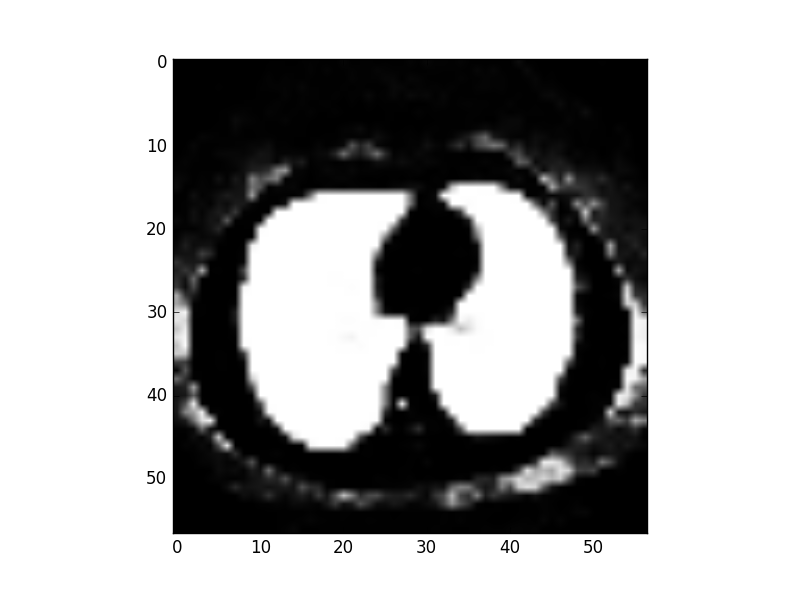
\includegraphics[width=\linewidth]{best_wel_lon.png}
    \caption{The result of using the full lung slice image (size 512x512) as input in the network.}
    \label{bestwellon}
\end{figure}

\begin{figure}
    \centering
    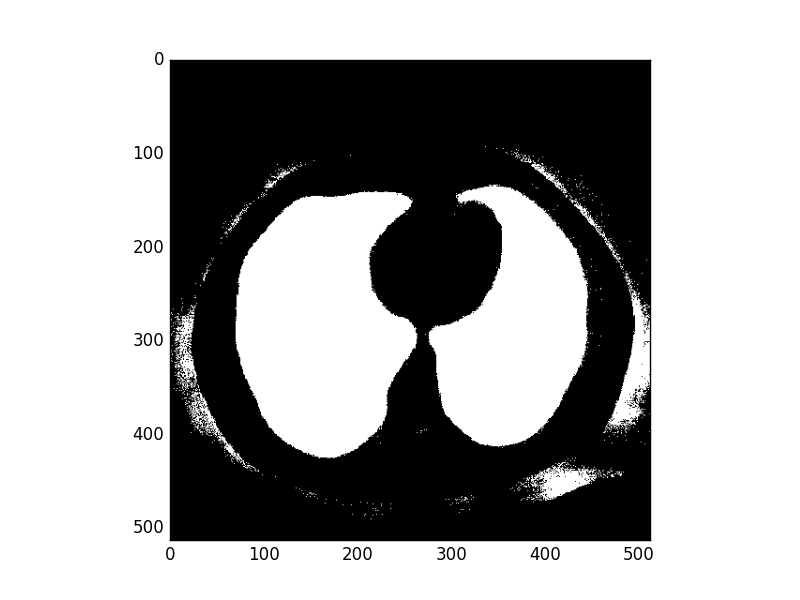
\includegraphics[width=\linewidth]{best_wel_prima.png}
    \caption{The result after performing shift-and-stitch.}
    \label{bestwelprima}
\end{figure}

\subsubsection{Nodule detection with Fully Convolutional Networks}
\label{sec:fcn}
We employ the exact same technique for nodule detection. The only difference is in the labels. Whereas we use the segmentation masks as the labels in the lung segmentation task, we now use nodule masks. We parsed the annotations.csv file and from this generated 3D masks that can be used as labels in the fully convolutional network. One extra challenge here is the extreme class imbalance. Even in the lung segmentation task, the class imbalance was something that we could not ignore. In that task, we employed class balancing by enforcing our minibatches to have a 50/50 split in terms of positive and negative samples. For the nodule detection task, this is harder, since we have even less positive samples. Even with data augmentation, the amount of positive samples is still too few. We therefore chose to create a minibatch split of 80/20 percent. This worked rather well for training. Patch-wise validation on a balanced test set also creates rather good results with a recall of 0.98 and a precision of 0.89. However, in the test set the balance is completely different. This causes the score metrics to look different. Our recall drops to 0.77 and our Dice score drops to 0.0006, indicating exceptionally bad results. We expect this problem to be due to the huge class imbalance. Possible approaches to tackle this problem is by trying different class balance ratios, or by only training on pixels which are part of the lungs (we currently train on all the possible pixels). Due to time constraints we were as of yet unable to get this method to work completely, as trying different training schemes is very time consuming. We will continue working on it during the next week since we can also use this method for false positive reduction. 

\subsection{Extracting candidates using Laplacian of Gaussian}
We used a second approach for detection lung nodule candidates which is the more conventional approach of using their blob-like structure. The first step is applying the lung segmentation as a mask on the lung CT images to reduce the search space to the actual lungs. The algorithm for the actual candidate detection is as follows:

\begin{itemize}
\item Apply two different sized Laplacian of Gaussian (LoG) filters. A LoG filter is circular-symmetric and thus widely used for blob detection, but has a maximum response to a particular blob size. We combined two filters with normalized kernels (IS THIS NORMALIZED?), the first with $\sigma = 3$ and \emph{kernel extent} = 7 and the second with $\sigma = 5$ and \emph{kernel extent} = 11 CHECK VALUES. We chose these parameters based on the paper of Van de Leemput et al. \cite{leemput}, who used LoG filters for pulmonary nodule detection in the \emph{ANODE09} challenge.
\item Take the pixel-wise maximum of the results of the LoGs to combine them to one result.
\item Threshold the resulting image with value THRESHOLDVALUEAFTERLOGS. See Figure \ref{figure:LoGresult} for an example result. This value is established by sampling the values of known nodules and healthy lung tissue.
	\begin{figure}[h]
	\centering
	{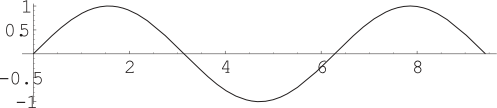
\includegraphics[width=0.7\linewidth]{./figure.png}}
	\caption{The thresholded image after taking the maximum of the two LoGs. \label{figure:LoGresult}}
	\end{figure}
\item Do a connected component analysis on the resulting image, and select only components with values between CONNECTEDCOMPONENTSVOLUMEVALUES. This identifies the initial candidates. See Figure \ref{figure:conncomp} for an example result.
	\begin{figure}[h]
	\centering
	{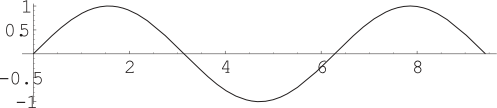
\includegraphics[width=0.7\linewidth]{./figure.png}}
	\caption{The result of applying a connected component analysis on the image shown in Figure \ref{figure:LoGresult}. \label{figure:conncomp}}
	\end{figure}
\item Threshold the resulting image again with value THRESHOLD2VALUE.
\item Apply dilation with a kernel of KERNELVALUE to increase the radius of the predicted candidates, i.e. predicted candidates will better correspond to lung nodule location. For example, if the prediction is only ten pixels removed from the actual nodule, this is really close in an image of 512 $\times$ 512 $\times$ \textit{ amount of slices} pixels. We still want this candidate to match with the ground truth.  See Figure \ref{figure:dilationresult} for an example result.
	\begin{figure}[h]
	\centering
	{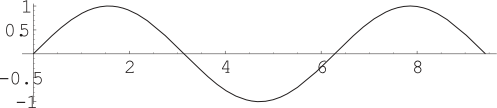
\includegraphics[width=0.7\linewidth]{./figure.png}}
	\caption{An example result after applying dilation. \label{figure:dilationresult}}
	\end{figure}
\end{itemize}

% Experiments
%\section{Experiments}\label{sec:experiments}

% Results
\section{Results}\label{sec:results}
\subsection{Candidate segmentation using the FCN}
As already noted in section \ref{sec:fcn} we managed to get a very good patch-wise score on a balanced validation set (recall of 0.98 and precision of 0.89), but due to the huge amount of negative pixels in the unbalanced test set, it performed very poorly as it classified a lot of negative pixels as positive. An example of a result is shown in figure \ref{figure:nodules}. This version of the network achieved a recall of 0.77 with and std of 0.33. The dice score was 0.006. 

\begin{figure}[h]
	\centering
	{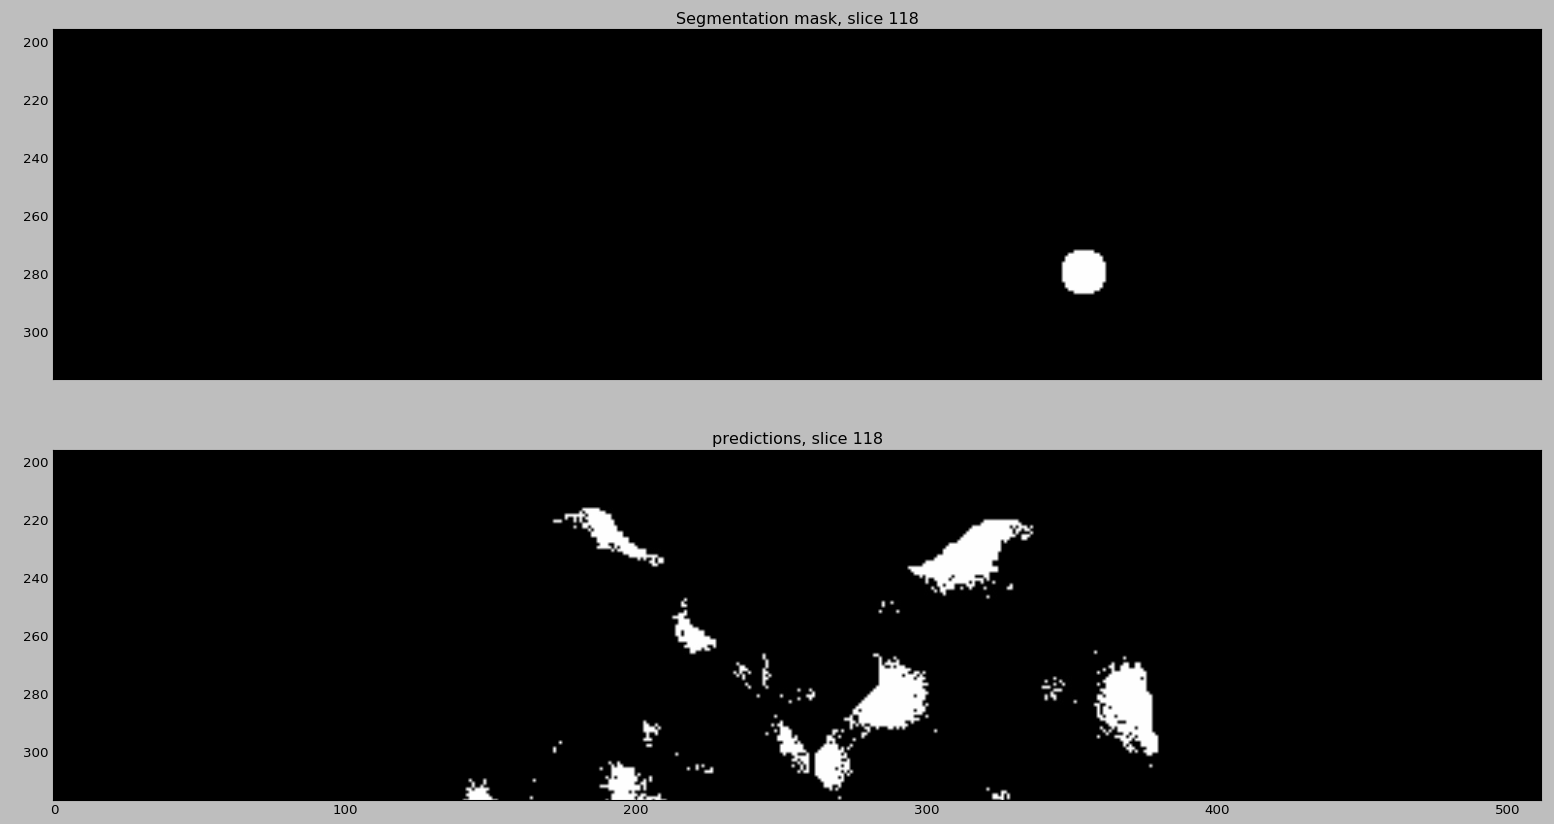
\includegraphics[width=0.7\linewidth]{./niet_zo_goed.png}}
	\caption{The upper image shows the nodule mask, the lower image shows the result of the FCN. \label{figure:nodules}}
\end{figure}

\subsection{Candidate extraction using Laplacian of Gaussian}
The results are based on the first 30 (AMOUNT) images in subset 9 of the dataset. The results are evaluated using the recall of the ground truth candidates given for this phase of the assignment, compared to our predicted nodule candidates. The reason that the results are only examined on SUBSET images is that this method is very time consuming (over ten minutes per image) and we continued tuning parameters and thereby improving our recall score relatively close to the deadline.

The average recall obtained by this method is MEANRECALLSCORE, with a standard deviation of STDRECALLSCORE. This score is relatively low, especially considering the high standard deviation. Additionally, increasing the recall drastically increased the total amount of predicted candidates which means there are a lot of false positives. However, the main goal of this method is to include all nodules in our candidates. Thus, it was important to reach a recall as high as possible, and we will worry about reducing the false positives later.

% Discussion
\section{Discussion}\label{sec:discussion}


\appendix
\section{Contributions}
\textbf{Luc Nies:} Final adjustments to the fully convolutional network so that it worked on the lung segmentation. Created the FCN pipeline, tested a lot of possible network and input parameters. Final adjustments to shift and stitch, and reading in of data. Wrote about the network architecture, parts of the nodule detection with FCN section and FCN conclusion.\\
\\
\textbf{Tom van de Poll:} \\
\\
\textbf{Harmen Prins:} \\
\\
\textbf{Steven Reitsma:} Helped building the fully convolutional network to work correctly. Fixed buggy shift and stitch method. Created 3D nodule masks. Wrote report sections on fully convolutional network. \\
\\
\textbf{Inez Wijnands:} Contributed to creating the MeVisLab candidate detection method using blob detection. Wrote introduction section and sections on the conventional approach in report.

% References should be produced using the bibtex program from suitable
% BiBTeX files (here: strings, refs, manuals). The IEEEbib.bst bibliography
% style file from IEEE produces unsorted bibliography list.
% -------------------------------------------------------------------------
\bibliographystyle{IEEEbib}

\begin{thebibliography}{}
\bibitem{long}
J. Long, E. Shelhamer \& T. Darrell (2015). Fully convolutional networks for semantic segmentation. \emph{Proceedings of the IEEE Conference on Computer Vision and Pattern Recognition}: 3431--3440.

\bibitem{simonyan}
K. Simonyan \& A. Zisserman (2014). Very deep convolutional networks for large-scale image recognition. \emph{arXiv:1409.1556}

\bibitem{leemput}
S. van de Leemput, F. Dorssers \& B.E. Bejnordi (2015). A novel spherical shell filter for reducing false positives in automatic detection of pulmonary nodules in thoracic CT scans. \emph{Proceedings SPIE Medical Imaging, 9414}:94142P.

\end{thebibliography}



\end{document}
